% \RequirePackage{currfile} 
\documentclass{beamer}

\mode<presentation> {

%\usetheme{default}
%\usetheme{AnnArbor}
%\usetheme{Antibes}
%\usetheme{Bergen}
%\usetheme{Berkeley}
\usetheme{Berlin} %+
%\usetheme{Boadilla}
%\usetheme{CambridgeUS} %-
%\usetheme{Copenhagen}
%\usetheme{Darmstadt}
%\usetheme{Dresden}
% \usetheme{Frankfurt}
%\usetheme{Goettingen}
%\usetheme{Hannover}
%\usetheme{Ilmenau}
%\usetheme{JuanLesPins}
%\usetheme{Luebeck}
% \usetheme{Madrid}      
%\usetheme{Malmoe}
%\usetheme{Marburg}
%\usetheme{Montpellier}
%\usetheme{PaloAlto}
%\usetheme{Pittsburgh}
% \usetheme{Rochester} %min
%\usetheme{Singapore}
%\usetheme{Szeged}
%\usetheme{Warsaw}

% As well as themes, the Beamer class has a number of color themes
% for any slide theme. Uncomment each of these in turn to see how it
% changes the colors of your current slide theme.

%\usecolortheme{albatross}
%\usecolortheme{beaver}
%\usecolortheme{beetle}
%\usecolortheme{crane}
%\usecolortheme{dolphin}
%\usecolortheme{dove}
% \usecolortheme{fly}
%\usecolortheme{lily}
%\usecolortheme{orchid}
% \usecolortheme{rose}
% \usecolortheme{seagull}
%\usecolortheme{seahorse}
\usecolortheme{whale}
%\usecolortheme{wolverine}

%\setbeamertemplate{footline} % To remove the footer line in all slides uncomment this line
%\setbeamertemplate{footline}[frame number] % To replace the footer line in all slides with a simple slide count uncomment this line

\setbeamertemplate{navigation symbols}{} % To remove the navigation symbols from the bottom of all slides uncomment this line

\setbeamercovered{transparent} % Fait apparaître les animations en grisé (utile pour la conception, mais peut être commenté lors de la remise du document final)

% Pour utiliser une police à empattements partout
\usefonttheme{serif}

% Pour rajouter la numérotation des frames dans les pieds de page
\newcommand*\oldmacro{}%
\let\oldmacro\insertshorttitle%
\renewcommand*\insertshorttitle{%
  \oldmacro\hfill%
  \insertframenumber\,/\,\inserttotalframenumber}

}


\usepackage[T2A]{fontenc}                   %!? закрепляет внутреннюю кодировку LaTeX
\usepackage[utf8]{inputenc}                 %!  закрепляет кодировку utf8
\usepackage[english,russian]{babel}         %!  подключает русский и английский
\usepackage[margin=1.7cm]{geometry}         %!  фиксирует оступ на 2cm

\usepackage[unicode, pdftex]{hyperref}      %!  оглавление для панели навигации по PDF-документу + гиперссылки

\usepackage{amsthm}                         %!  newtheorem и их сквозная нумерация
\usepackage{hypcap}                         %?  адресация на картинку, а не на подпись к ней
\usepackage{caption}                        %-  позволяет корректировать caption 
\usepackage{fancyhdr}                       %   добавить верхний и нижний колонтитул
\usepackage{wrapfig}                        %!  обтекание таблиц и рисунков

\usepackage{amsmath}                        %!  |
\usepackage{amssymb,textcomp, esvect,esint} %!  |важно для формул 
\usepackage{amsfonts}                       %!  математические шрифты
\usepackage{mathrsfs}                       %  добавит красивые E, H, L
\usepackage{ulem}                           %!  перечеркивание текста
\usepackage{abraces}                        %?  фигурные скобки сверху или снизу текста
\usepackage{pifont}                         %!  нужен для крестика
\usepackage{cancel}                         %!  аутентичное перечеркивание текста
\usepackage{esvect}                         %  добавит вектора стрелочками

\usepackage{graphicx}                       %?  графическое изменение текста
\usepackage{indentfirst}                    %   добавить indent перед первым параграфом
\usepackage{xcolor}                         %   добавляет цвета
\usepackage{enumitem}                       %!  задание макета перечня.

\usepackage{booktabs}                       %!  добавляет книжные линии в таблицы
\usepackage{multirow}                       %   объединение ячеек в таблицах

\usepackage{tikz}                           %!  высокоуровневые рисунки (кружочек)

\usepackage{import}                         %   |
\usepackage{xifthen}                        %   |
\usepackage{pdfpages}                       %   | вставка рисунков pdf_tex
\usepackage{transparent}                    %   |

\setlength{\headheight}{12.52pt}            % избегать warning

\usepackage{media9}
\usepackage{animate}
\usepackage{enumitem}
\usepackage{threeparttable}
\usepackage{pifont}


\usepackage{import}
\usepackage{xifthen}
\usepackage{pdfpages}
\usepackage{transparent}

% \newcommand{\incfig}[1]{%
%     \def\svgwidth{\columnwidth}
%     \import{./figures/}{#1.pdf_tex}
% }

% \usepackage{circuitikz}

\newcommand{\vc}[1]{\mbox{\boldmath $#1$}}
\newcommand{\T}{^{\text{T}}}
\newcommand{\xmark}{\ding{55}}
\newcommand{\R}{\text{R}}
\newcommand{\const}{\text{const}}
\newcommand{\rot}{\text{rot}}
\renewcommand{\d}{\text{ d}}

\newcommand{\incfig}[1]{%
    % \def\svgwidth{}
    \import{../Figures/}{#1.pdf_tex}
}

\newcommand{\com}[1]{\textcolor{red}{#1}}

\newcommand{\progressbar}{%
	\pgfmathsetmacro{\slidewidth}{\paperwidth}
	\pgfmathsetmacro{\progressstep}{\paperwidth/\inserttotalframenumber}
	\pgfmathsetmacro{\progresspos}{(\insertframenumber - 0.5) * \progressstep}
	\begin{tikzpicture}[scale = 0.035, line width = 1ex]
		\node[inner sep=0pt] (cat) at (\progresspos,0)	{
\includegraphics[width=20pt]{cat.png}};
		\path[red] (0,0) -- (\slidewidth,0);
	\end{tikzpicture}
}

\makeatletter
\setbeamertemplate{footline}
{
\hfill \progressbar%
  \leavevmode%
  \hbox{%
  \begin{beamercolorbox}[wd=.433333\paperwidth,ht=2.25ex,dp=1ex,center]{section in head/foot}%
    \usebeamerfont{author in head/foot}\insertshortauthor~~\beamer@ifempty{\insertshortinstitute}{}{(\insertshortinstitute)}
  \end{beamercolorbox}%
  \begin{beamercolorbox}[wd=.333333\paperwidth,ht=2.25ex,dp=1ex,center]{section in head/foot}%
    \usebeamerfont{title in head/foot}\insertshorttitle
  \end{beamercolorbox}%
  \begin{beamercolorbox}[wd=.333333\paperwidth,ht=2.25ex,dp=1ex,right]{section in head/foot}%
    % \usebeamerfont{date in head/foot}\insertshortdate{}\hspace*{2em}
    % \insertframenumber{} / \inserttotalframenumber\hspace*{2ex} 
  \end{beamercolorbox}}%
  \vskip0pt%
}


\newcommand{\agemO}{$\Omega^{-1}$}

\title[Jacob's Ladder]{ Laboratory  research project on  \\ High Voltage Travelling Arc \\
Jacob's Ladder}
\author{Khoruzhii Kirill and Primak Eugene}
\institute[MIPT]
% \date{19 of December 2020}

\begin{document}
\date{12.19.2020}
\maketitle

\begin{frame}
\frametitle{To be discussed}
\tableofcontents
\end{frame}

\section{Motivation}

\section{Review}
% \frame{\begin{figure}[htbp]
	\centering
	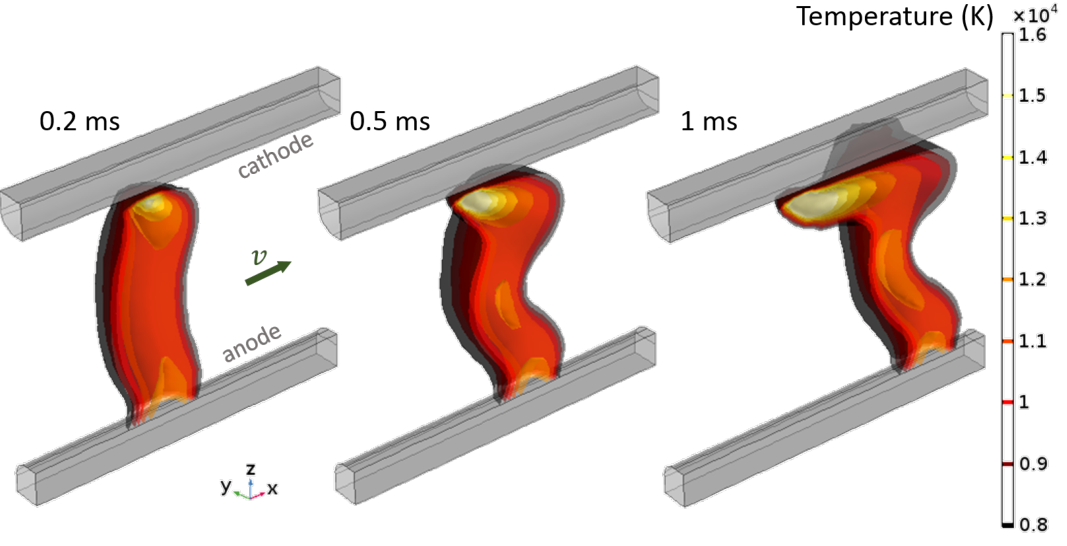
\includegraphics[width=0.65\textwidth]{images/phd_simulT.png}
	\caption*{Time evolution of the temperature distribution in the arc column}
	\label{phd}
\end{figure}

\footnotesize{
\begin{thebibliography}{99}
    \bibitem[APS]{p1}  M.Lisnyak Plasma Physics. Université Orléans, 2018. tel-01808258
\end{thebibliography}} \frametitle{Theoretical, numerical and experimental study of DC
% and AC electric arcs}}
% \frame{\begin{minipage}[b]{0.45\linewidth}
	\begin{figure}[htbp]
	\centering
	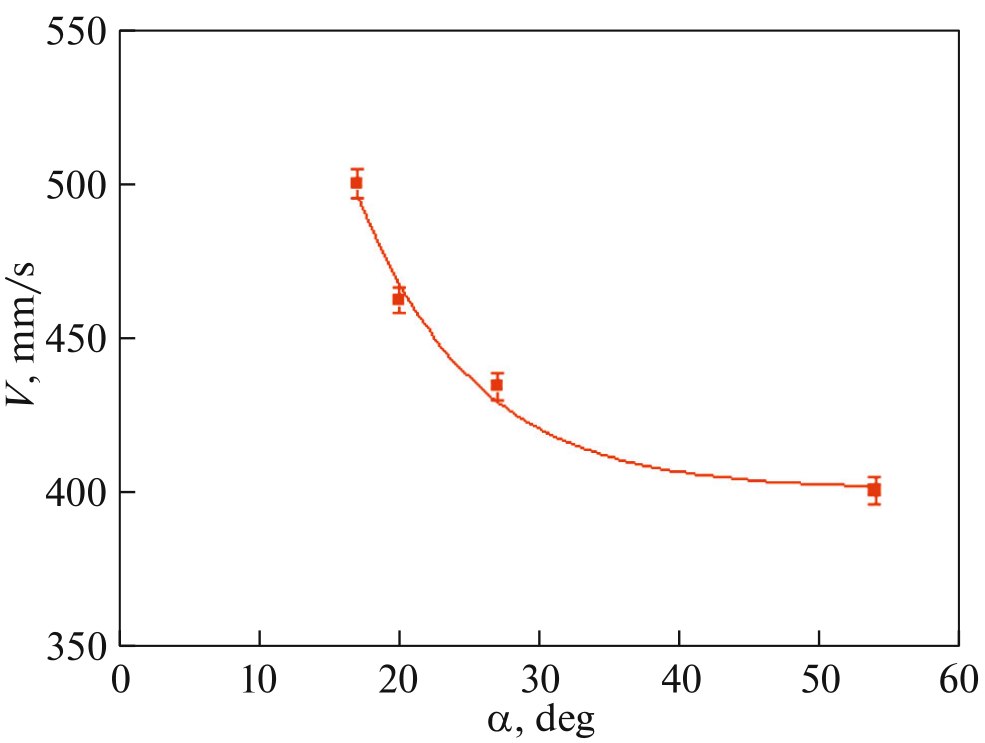
\includegraphics[width=1\textwidth]{images/almazova_vel.png}
	\caption*{}
	\label{alm_data}
	\end{figure}
\end{minipage}
\hfill
\begin{minipage}[b]{0.45\linewidth}

\end{minipage}

\footnotesize{
\begin{thebibliography}{99}
    \bibitem[APS]{p2}  K. I. Almazova et al. 2020 Plasma Vol. 90, No. 7, pp. 1076–1079
\end{thebibliography}

\begin{thebibliography}{99}
    \bibitem[APS]{p3}  Jindong Huo, JoAnne Ronzello et al. AIP Advances 10, 085324 (2020)
\end{thebibliography}
} \frametitle{Articles we have started with}}
% \frame{


\footnotesize{
\begin{thebibliography}{99}
    \bibitem[APS]{p3}  Jindong Huo, JoAnne Ronzello et al. AIP Advances 10, 085324 (2020)
\end{thebibliography}} \frametitle{Development of an arc root model for
% studying the electrode vaporization and its
% influence on arc dynamics}}

% \section{Theory}
% \frame{The formulas that are used to describe arc bulk plasma are taken from following work
{\footnotesize
\begin{thebibliography}{99}
    \bibitem[APS]{p1}  M.Lisnyak Plasma Physics. Université Orléans, 2018. tel-01808258
\end{thebibliography}}

\phantom{239}

Assuming quasi neutrality of the plasma, one obtains the Navier-Stokes equation for the whole gas:

\begin{equation}
\frac{\partial \rho \vc{v}}{\partial t} + \nabla \cdot \rho \vc{v} \otimes \vc{v} = - \nabla p - \nabla \hat{\pi},
\label{ppi}
\end{equation}

where $p$ is the total plasma pressure and $\hat{\pi}$ is the viscous \hyperlink{navier}{tensor}.

 \frametitle{Fluid plasma description}}
% \frame{In terms of \textit{Landau-Lifshitz. Theoretical physics. <<Hydrodynamics>>} concervation of energy of the plasma can be written as:

\begin{equation}
	p C_p \left(\frac{\partial T}{\partial t} + \vc{v} \cdot \nabla T\right) = - \nabla \cdot \vc{q} + Q_\text{JH} - Q_\text{rad},
\end{equation}
where  q, the energy flux, is presented with following formula:
 $$\vc{q} = - \lambda \nabla T - \left(\frac{5}{2}  + k_{T}\right) \frac{k_B T}{e} \vc{j}.$$ \frametitle{Energy conservation}}
% \frame{The continuity equation of the whole plasma can be obtained from the species mass conservation

\begin{equation}
	\frac{\partial p}{\partial t} + \nabla \cdot p \vc{v} = 0.
\end{equation}

The simplified Ohm's law shows that arc current:

\begin{equation}
	\vc{j} = \sigma \vc{E} + \frac{e D_e^T}{m_e T} \nabla T,
\end{equation}

where $D_e^T$ is the thermal diffusion coefficient. \frametitle{Laws of flows}}
% \frame{Due to the formula for charge density $\rho_e = e (Z n_i - n_e)$ the charge conversation might be written as:

\begin{equation}
	\nabla \cdot \vc{j} = 0 \hspace*{1 cm} \leadsto \hspace*{1 cm} \nabla \cdot \vc{j}.
\end{equation}

And useful Maxwell's equations:

\begin{equation}
	\nabla \times \vc{B} = \mu_0 \vc{j}
	\hspace*{3cm} \nabla \times \vc{A} = \vc{B},
\end{equation}
where A is vector potential. \frametitle{Charge conservation and Maxwell}}

% \section{Experiment}
% \frame{	\begin{figure}[htbp]
	\centering
	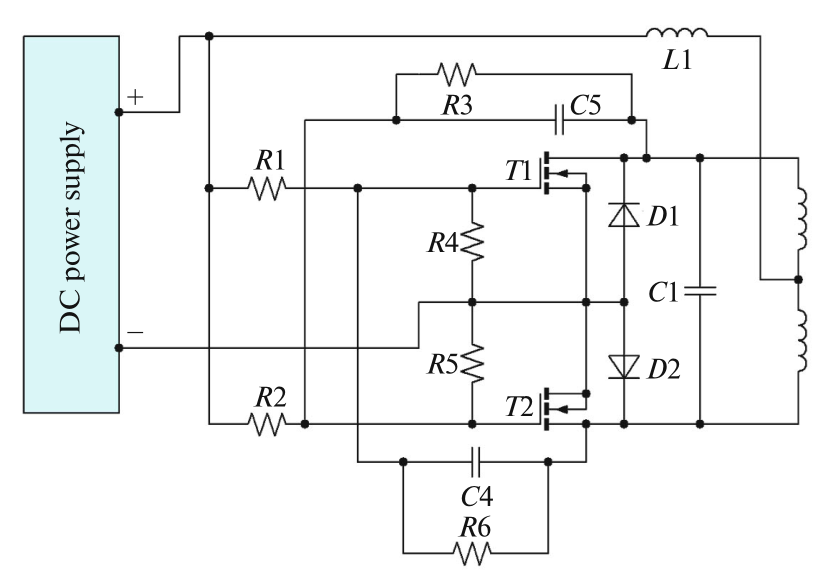
\includegraphics[width=0.6\textwidth]{images/almazova_circ.png}
	\caption*{ZVC-driver}
	\label{alm_circ}
	\end{figure}

\footnotesize
\begin{thebibliography}{99}
    \bibitem[APS]{p2}  K. I. Almazova et al. 2020 Plasma Vol. 90, No. 7, pp. 1076–1079
\end{thebibliography} \frametitle{Choosing high a voltage circuit}}

% \frame{\begin{figure}[htbp]
	\centering
	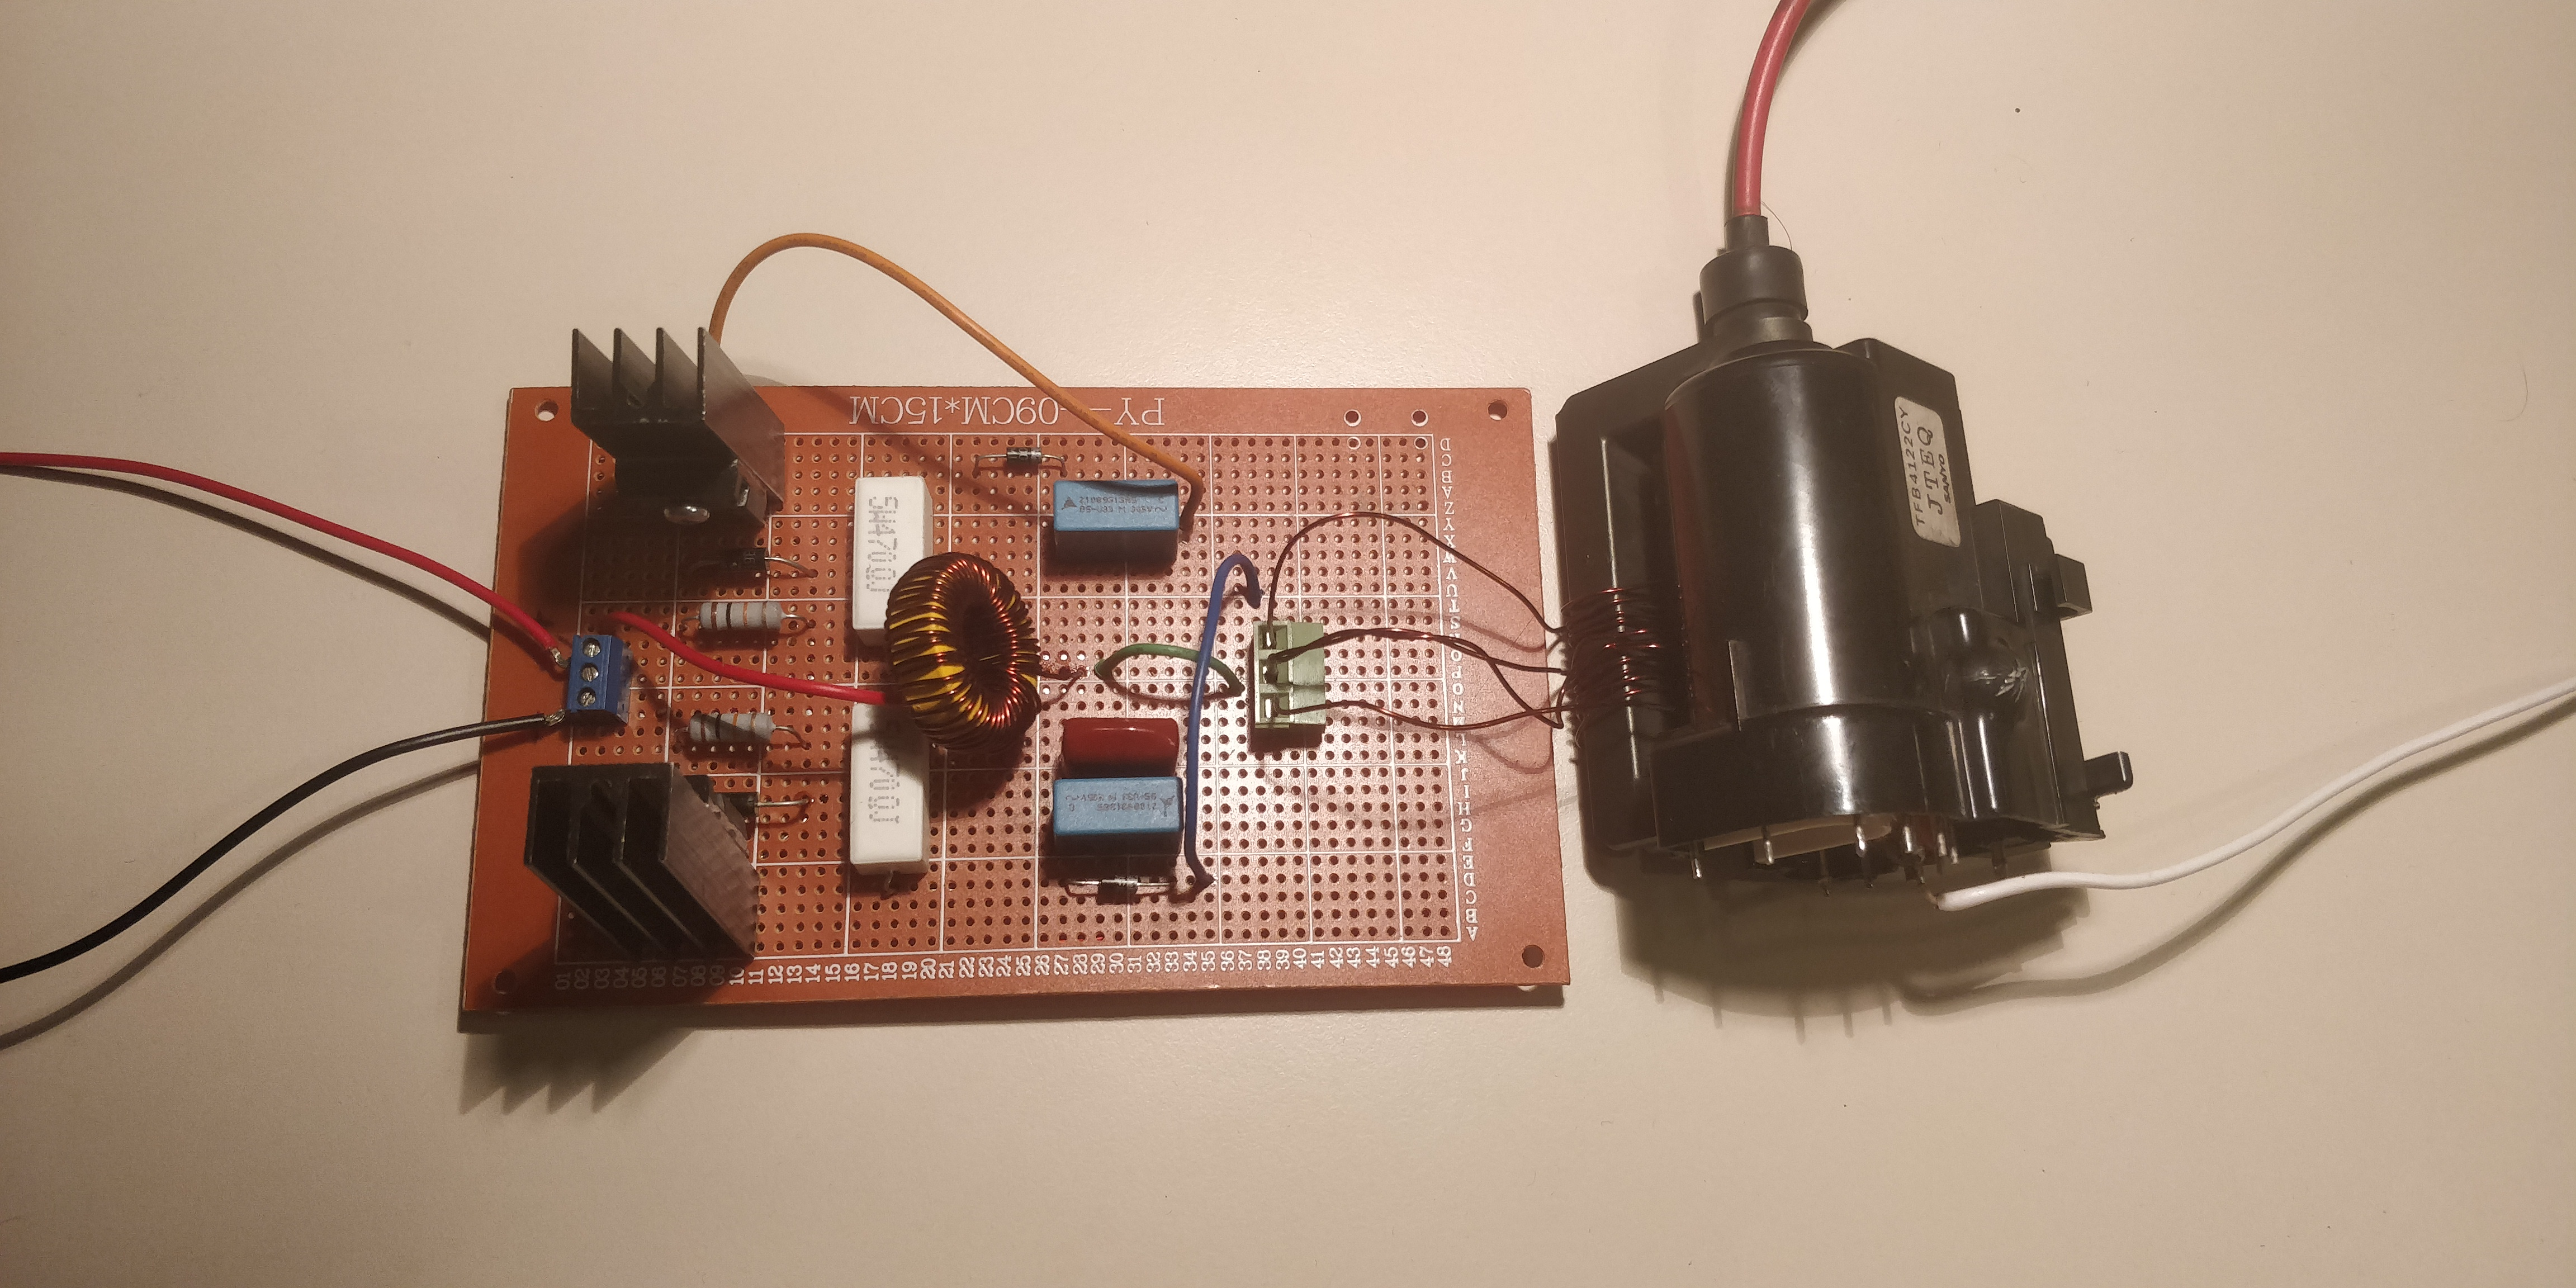
\includegraphics[width=0.95\textwidth]{images/circuit.jpg}
	\caption*{Circuit is connected to a transformator from an old TV}
	\label{circuit}
\end{figure} \frametitle{The circuit was soldered}}
% \frame{\begin{figure}[htbp]
	\centering
	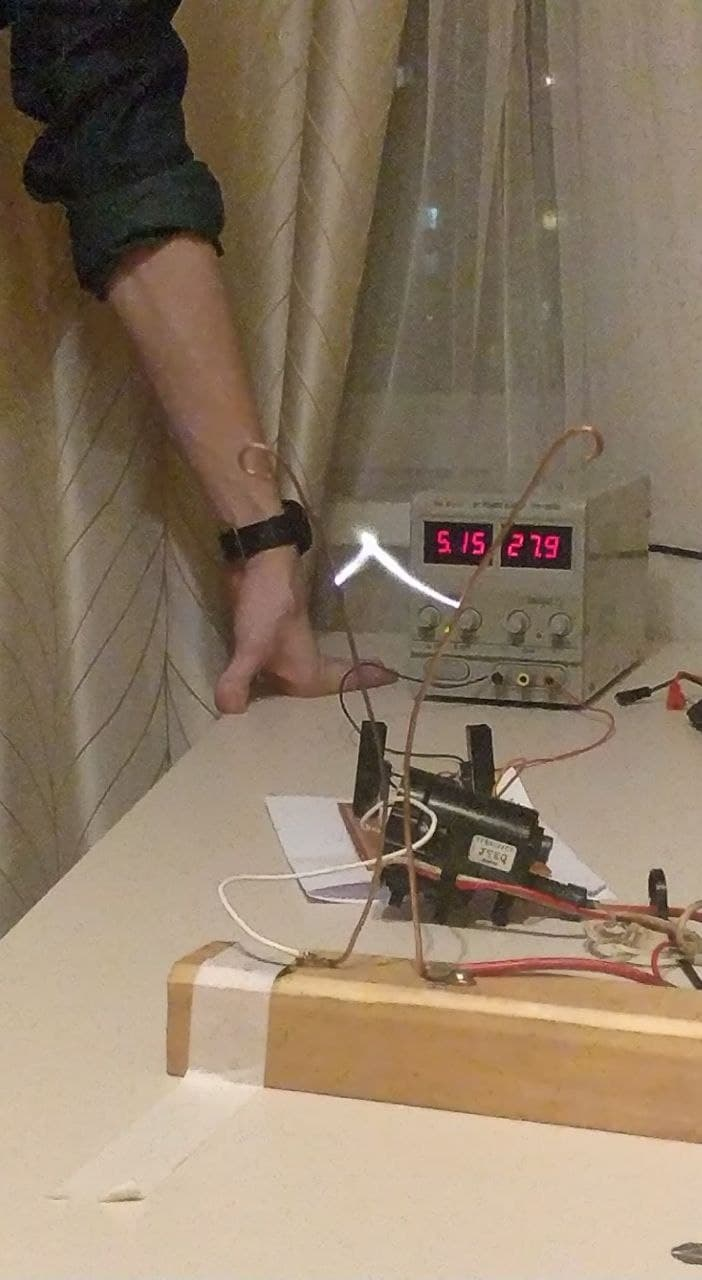
\includegraphics[width=0.27\textwidth]{images/v1.jpg}
	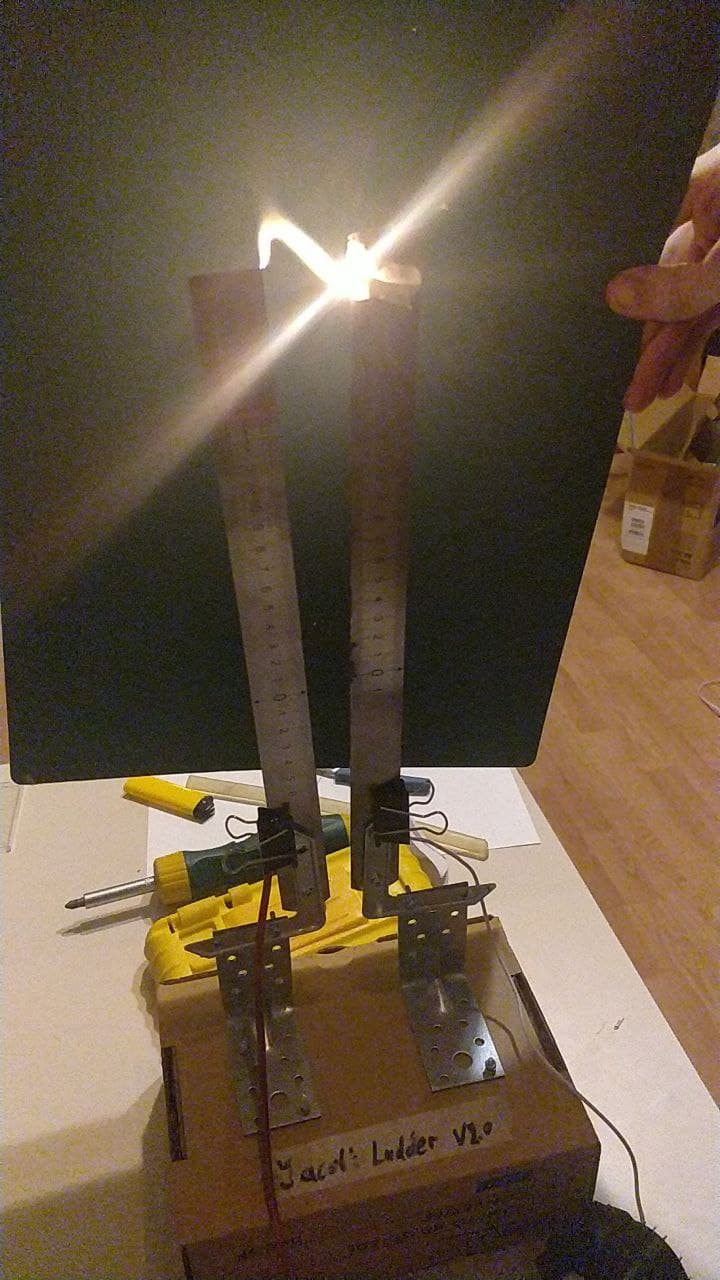
\includegraphics[width=0.27\textwidth]{images/v2.jpg}
	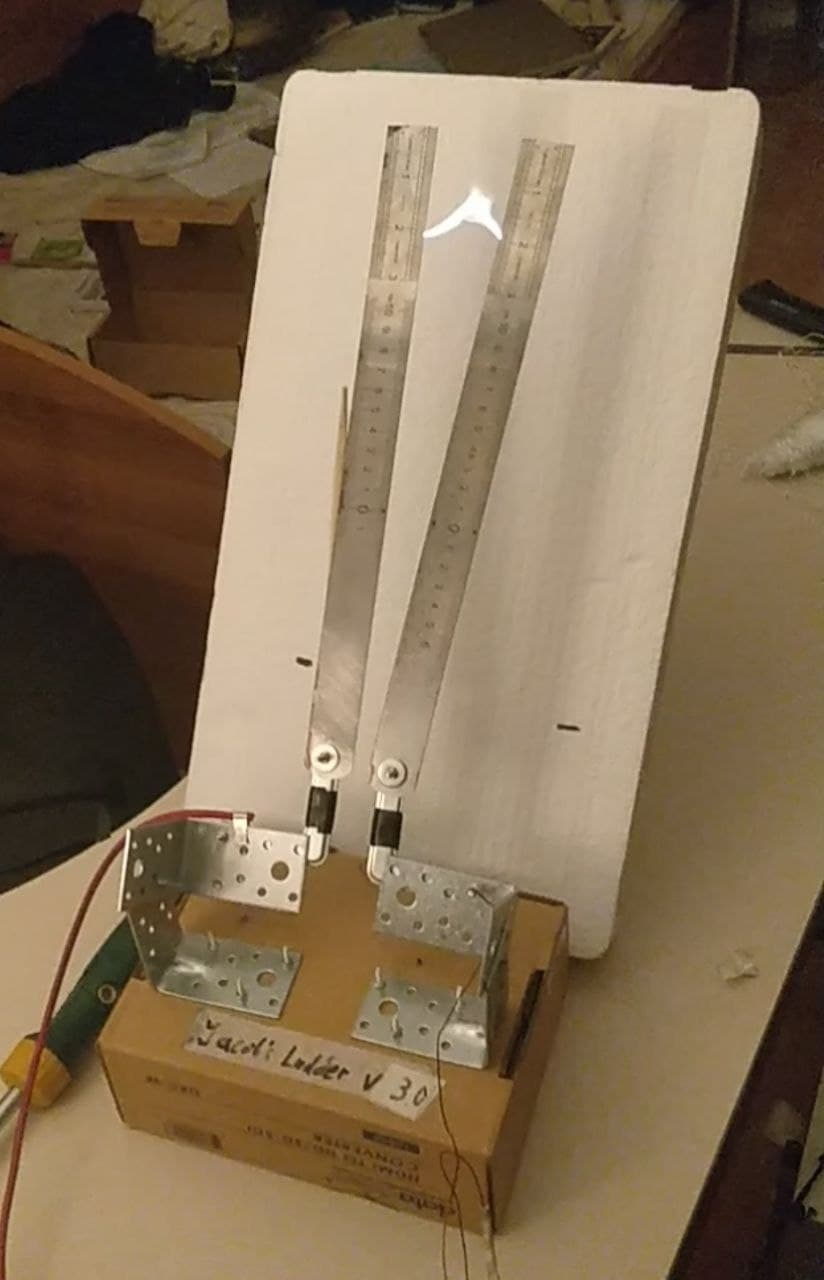
\includegraphics[width=0.27\textwidth]{images/v3.jpg}
	\caption*{All versions in a row: v1 -- first attempt; v2 -- supports opening; v3 -- supports rotation.}
	\label{circuit}
\end{figure} \frametitle{Evolution of experimental setup}}

\section{Data}
\frame{% \begin{figure}[htbp]
%     \incfig{1}
% \end{figure}



% \begin{minipage}[c]{0.2\textwidth}
%     \begin{align*}
%     Oy \in \text{ plane of electrodes},\ \beta = \angle (\vc{g}, Oy) \\
%     \alpha \text{ -- opening angle,} \
%     \beta \text{ -- rortation angle,} \\
%      .
%     \end{align*}
% \end{minipage}
% \hfill

\begin{figure}[h]
\centering
 \animategraphics[loop,controls,width=0.3\textwidth]{20}{../gifs/g4/}{1}{200}
    %\caption{}
    %\label{fig:}
\end{figure}


}
% \frame{

\begin{figure}[h]
\centering
 \animategraphics[loop,controls,width=0.5\textwidth]{20}{../gifs/g2/}{770}{1228} 
\end{figure}


}
% \frame{
13.
Next, we measured the dependence of the arc coordinate y on the time at different 
opening angles (between electrodes) 
and rotation angle (between electrodes plane and Gravitational acceleration). 
The coordinate was correspondingly measured along the electrodes. 

Using Python, the alpha and beta values ​​were taken from the captured videos, as well as the arc coordinate.


14.
First of all, we confirmed the hypothesis that the reason for the rise of the arc is the Archimedes force. The graph shows the dependence of the arc rise speed on time with different values of the rotation angles beta. Average values ​​are highlighted. In the limit of 90 degrees beta, no arc movement is observed. 
Thus, the hydrodynamic nature of motion is confirmed.



15.
In the article that inspired us, it was argued that at some point, the speed of the arc comes to a constant value. Sufficiently accurate measurements are required to verify this. The graph shows the results of the dependence of the arc coordinate on the time with different opening angles alpha.

16.
So, at some values ​​of the alpha a mode with a constant speed is reached.
I would like to see the plot of the speed versus time.
It is shown on the slide for an alpha value of 34 degrees.
The speed becomes constant, indeed.


17.
As we measured, the constant speed mode is not achieved at an angle of less than 14 degrees, which is clearly shown in the graph. Arc break occurs before stabilization on the top graph.


18.
For various values ​​of the opening angle, we've founded the average value of the speed after stabilization.


19.
This allowed us to plot the dependence of the average arc speed on the opening angle. The curve here is just a spline approximation. So, it can be seen that with increasing angle the constant speed increases.


20.
This clearly contradicts the values ​​obtained in the referenced earlier article,
which undoubtedly deserves attention. 
Note that the article did not stipulate the repeatability of the experiments, it is not known whether averaging over different launches took place, perhaps this is the reason.


21. 
To sum up, 

We worked through theory that is enough for modelling high
voltage electric arc.

We built the experimental setup and gathered and processed
the data.

We shoved that the key role in up movement of the arc is
presented by pressure gradient.

We measured dependence of the average stabilized velocity to
the opening angle, that conflicts with the results of Almazova's
article.

Algorithms}
% \frame{\begin{figure}[htbp]
	\centering
	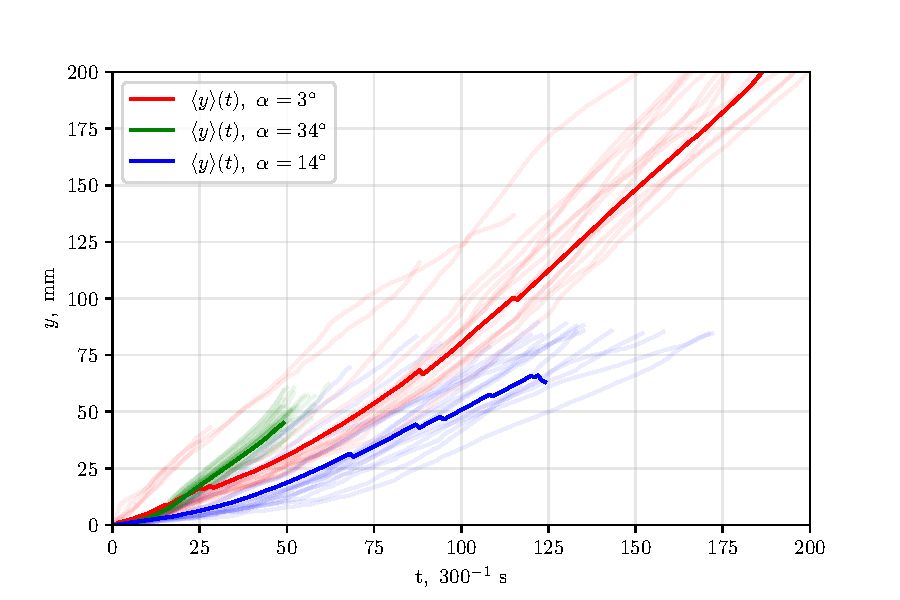
\includegraphics[width=0.8\textwidth]{figures/2)_y(t).pdf}
	\caption{Dependence of $ y (t) $ at different opening angles $\alpha$.}
	\label{fig:label}
\end{figure} \frametitle{With high speed camera}}
% \frame{\begin{figure}[htbp]
	\centering
	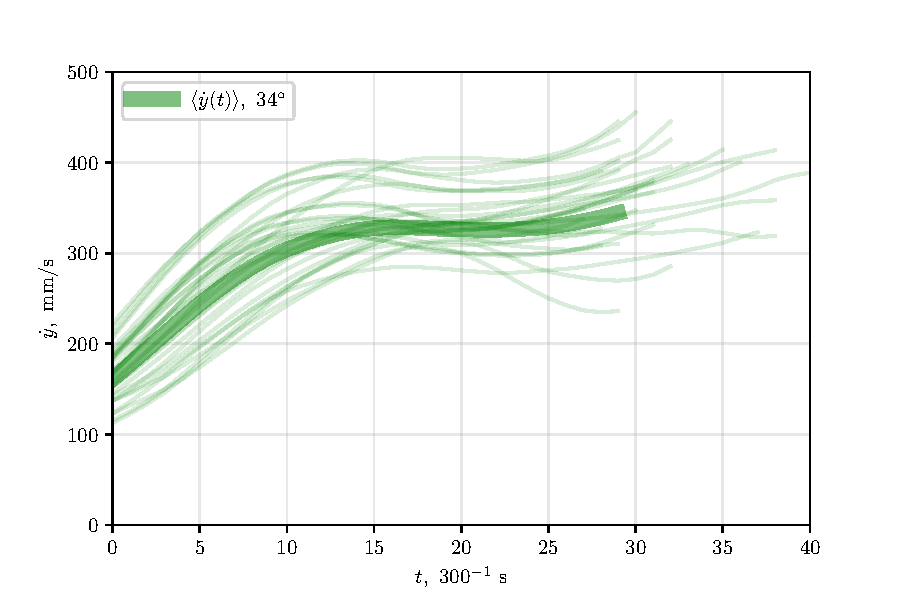
\includegraphics[width=0.8\textwidth]{figures/3)_dot_y_34.pdf}
	\caption{Dependence of $ y (t) $ at different opening angles $\alpha$.}
	\label{fig:label}
\end{figure} \frametitle{With high speed camera}}
% \frame{\begin{figure}[htbp]
	\centering
	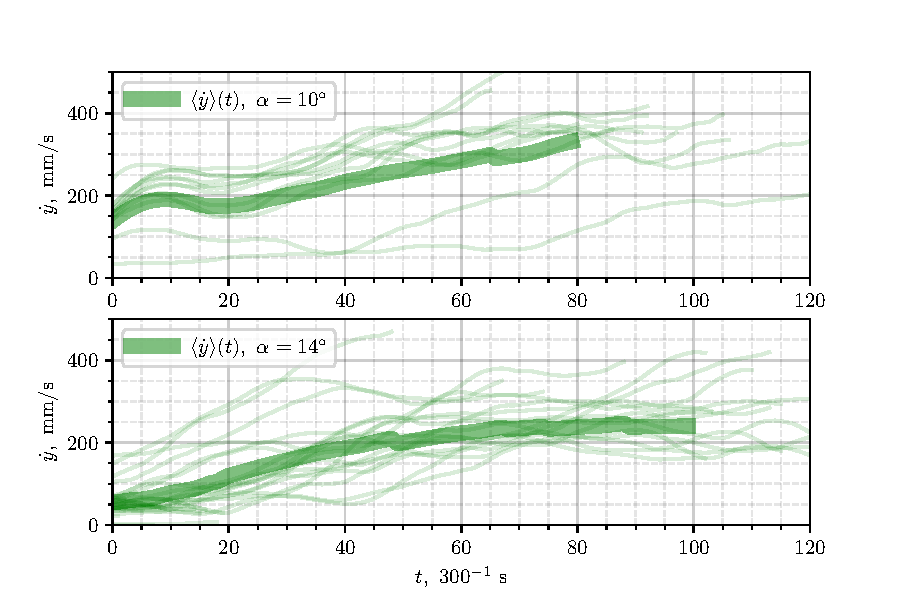
\includegraphics[width=0.8\textwidth]{figures/4,5)_dot_y_[10,14].pdf}
	\caption{Dependence of the velocity of arc rise $\langle \dot{y}\rangle$ on time $t$ at different opening angles.}
	\label{fig:label}
\end{figure} \frametitle{With high speed camera}}
% \frame{\begin{figure}[htbp]
	\centering
	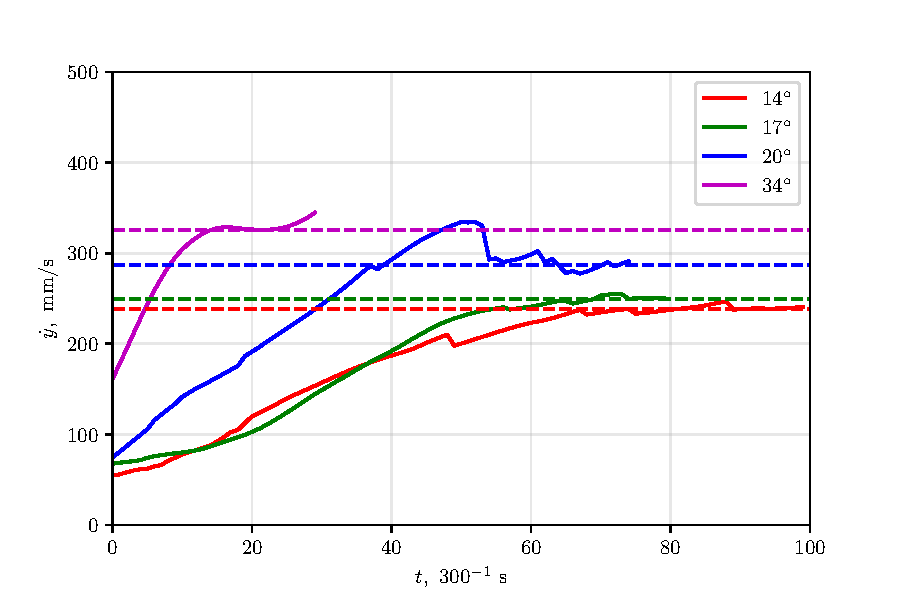
\includegraphics[width=0.8\textwidth]{figures/6)_vs_lines.pdf}
	\caption{Dependence $\dot{y} (\alpha)$, dashed line corresponds to the average value $\langle \dot{y}\rangle (\alpha)$ over the considered interval.}
	\label{fig:label}
\end{figure} \frametitle{With high speed camera}}
% \frame{\begin{figure}[htbp]
	\centering
	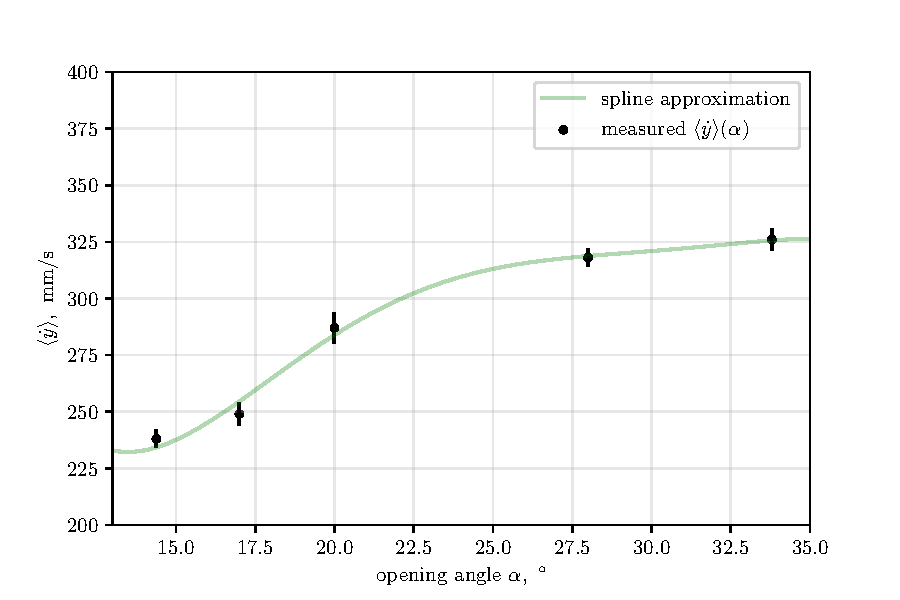
\includegraphics[width=0.8\textwidth]{figures/7)_mvs.pdf}
	\caption{Dependence of the velocity of arc rise $\langle \dot{y}\rangle$ on the opening angle $\alpha$ between the electrodes.}
	\label{fig:label}
\end{figure} \frametitle{With high speed camera}}
% \frame{\begin{figure}[htbp]
	\centering
	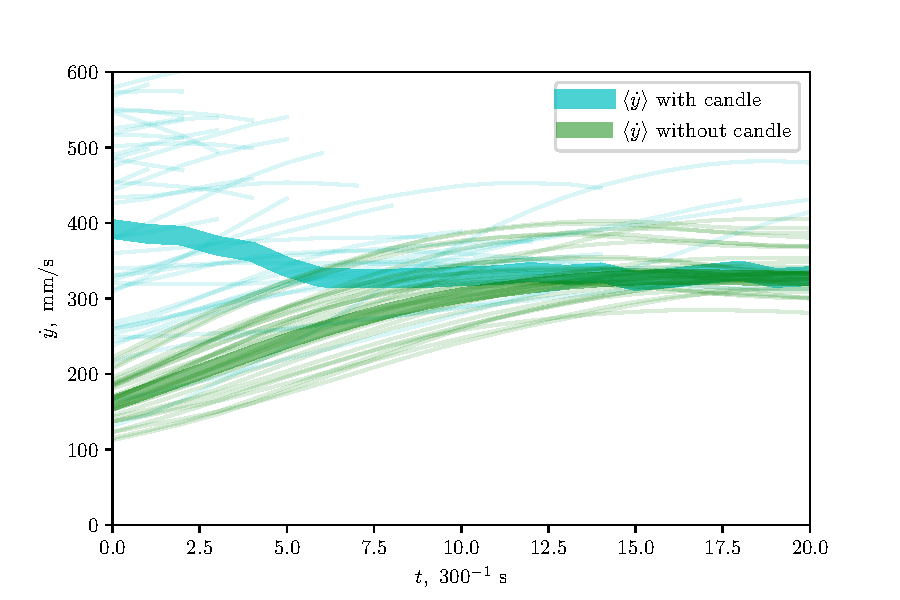
\includegraphics[width=0.8\textwidth]{figures/8)_candle_dot_y_a33.pdf}
	\caption{Dependence of the velocity of arc rise $\langle \dot{y}\rangle$ on time $t$ for the case with and without a candle.}
	\label{fig:label}
\end{figure} \frametitle{With high speed camera}} ########свеча


% \section{Conclusion}


% \frame{\frametitle{Thank you for your attention!}}

% \frame{In equation \eqref{ppi} $p$ and $\pi$ present these formulas:

\begin{align*}
	p& = \sum_a p_a = \sum n_a k_B T_a \\
	\hat{\pi}_{i,j}& = -\mu \left[\left(\frac{\partial v_i}{\partial x_j} + \frac{\partial v_j}{\partial x_i}\right) - \frac{2}{3} \nabla \cdot \vc{v} \delta_{i j}\right]
	\label{navier}
\end{align*} \frametitle{Additions}}

\end{document}